\documentclass[12pt,a4paper]{article}
\usepackage[margin=1in]{geometry}
\usepackage{amsmath, amssymb, amsthm}
\usepackage{algorithm}
\usepackage{algpseudocode}
\usepackage{titlesec}
\usepackage{graphicx}
\usepackage{xcolor}
\usepackage{tcolorbox}
\usepackage{hyperref}
\usepackage{listings}
\usepackage{fancyhdr}
\usepackage{enumitem}
\usepackage{tikz}
\usepackage{forest}

% Hyperref setup
\hypersetup{
    colorlinks=true,
    linkcolor=blue,
    urlcolor=blue,
    citecolor=red
}

% Color definitions
\definecolor{lightgray}{gray}{0.95}
\definecolor{darkgray}{gray}{0.3}
\definecolor{codegreen}{rgb}{0,0.6,0}
\definecolor{codegray}{rgb}{0.5,0.5,0.5}
\definecolor{codepurple}{rgb}{0.58,0,0.82}
\definecolor{backcolour}{rgb}{0.95,0.95,0.92}
\definecolor{javared}{rgb}{0.6,0,0}
\definecolor{javagreen}{rgb}{0.25,0.5,0.35}
\definecolor{javapurple}{rgb}{0.5,0,0.35}
\definecolor{javadocblue}{rgb}{0.25,0.35,0.75}

% Code listing style for Java
\lstdefinestyle{mystyle}{
    language=Java,
    backgroundcolor=\color{backcolour},
    commentstyle=\color{codegreen},
    keywordstyle=\color{javared}\bfseries,
    numberstyle=\tiny\color{codegray},
    stringstyle=\color{javapurple},
    basicstyle=\ttfamily\footnotesize,
    breakatwhitespace=false,
    breaklines=true,
    captionpos=b,
    keepspaces=true,
    numbers=left,
    numbersep=5pt,
    showspaces=false,
    showstringspaces=false,
    showtabs=false,
    tabsize=2,
    frame=single,
    rulecolor=\color{black}
}

\lstset{style=mystyle}

% Title formatting
\titleformat{\section}{\normalfont\Large\bfseries\color{blue}}{\thesection}{1em}{}
\titleformat{\subsection}{\normalfont\large\bfseries\color{darkgray}}{\thesubsection}{1em}{}
\titleformat{\subsubsection}{\normalfont\normalsize\bfseries\color{black}}{\thesubsubsection}{1em}{}

% Header and footer
\pagestyle{fancy}
\fancyhf{}
\rhead{Closest Pair Sum Algorithm}
\lhead{Algorithm Analysis}
\cfoot{\thepage}

% Theorem environments
\newtheorem{theorem}{Theorem}
\newtheorem{lemma}{Lemma}
\newtheorem{definition}{Definition}

% Title page setup
\title{\textbf{ClosestPairFinder Algorithm:\\Complete Analysis and Implementation}}
\author{
    \textbf{Divide and Conquer Approach}\\
    \textit{Finding the Pair with Sum Closest to Target}\\
    \vspace{0.5em}
    \small Algorithm Implementation and Analysis
}
\date{\today}

\begin{document}

\maketitle

\begin{center}
\rule{\textwidth}{2pt}
\vspace{0.5em}
\large \textbf{Comprehensive Algorithm Documentation}
\vspace{0.5em}
\rule{\textwidth}{1pt}
\end{center}

\vspace{2em}

\begin{abstract}
This document provides a comprehensive analysis of the ClosestPairFinder algorithm, which implements a divide-and-conquer approach to find two numbers in an array whose sum is closest to a given target value. The analysis includes detailed explanation of the algorithm's structure, complexity analysis, step-by-step execution examples, and theoretical foundations. The algorithm achieves O(n log n) time complexity through efficient sorting and recursive subdivision of the problem space.
\end{abstract}

\vspace{1em}
\tableofcontents
\newpage

\section{Problem Statement and Definition}

\subsection{Problem Description}
\begin{tcolorbox}[colback=blue!5!white,colframe=blue!50!black,title=\textbf{Closest Pair Sum Problem}]
Given an array of $n$ integers and a target value $T$, find two distinct elements $a[i]$ and $a[j]$ (where $i \neq j$) such that $|a[i] + a[j] - T|$ is minimized.

\textbf{Input:}
\begin{itemize}
    \item Array $A[0..n-1]$ of integers
    \item Target sum $T$
\end{itemize}

\textbf{Output:}
\begin{itemize}
    \item Pair $(a[i], a[j])$ that minimizes $|a[i] + a[j] - T|$
\end{itemize}

\textbf{Example:} For array $[10, 2, 7, 3, 1, 9, 4]$ and target $T = 11$, the closest pair is $(2, 9)$ with sum $11$.
\end{tcolorbox}

\subsection{Mathematical Formulation}

\begin{definition}[Closest Pair Sum]
Let $A = \{a_1, a_2, \ldots, a_n\}$ be a set of integers and $T$ be the target sum. The closest pair sum problem seeks to find indices $i, j$ such that:
\[
\min_{1 \leq i < j \leq n} |a_i + a_j - T|
\]
\end{definition}

\section{Algorithm Overview and Strategy}

\subsection{High-Level Approach}

The ClosestPairFinder algorithm employs a divide-and-conquer strategy with the following key phases:

\begin{enumerate}[itemsep=0.5em]
    \item \textbf{Preprocessing:} Sort the input array to enable efficient searching
    \item \textbf{Divide:} Recursively split the array into left and right halves
    \item \textbf{Conquer:} Find closest pairs in three scenarios:
    \begin{itemize}
        \item Both elements from the left half
        \item Both elements from the right half  
        \item One element from each half (cross pair)
    \end{itemize}
    \item \textbf{Combine:} Select the best pair among the three candidates
\end{enumerate}

\subsection{Algorithm Structure}

\begin{center}
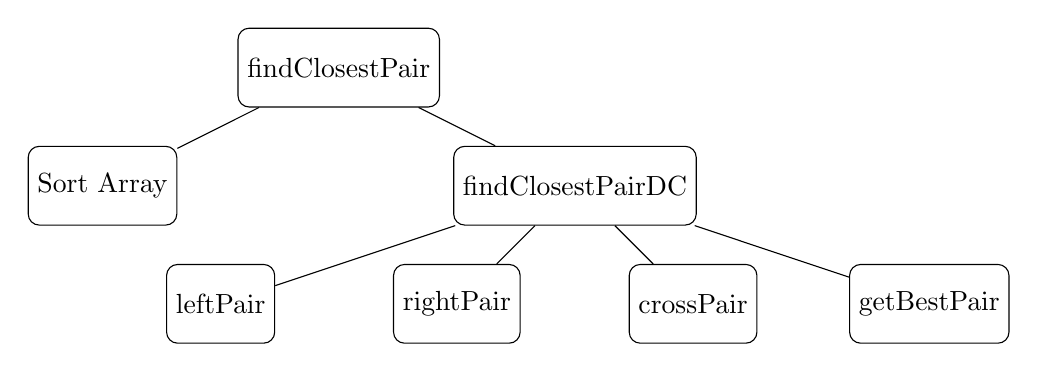
\begin{tikzpicture}[
    level/.style={sibling distance=60mm/#1},
    every node/.style={draw, rounded corners, minimum height=1cm, text centered}
]
\node {findClosestPair}
    child {node {Sort Array}}
    child {node {findClosestPairDC}
        child {node {leftPair}}
        child {node {rightPair}}
        child {node {crossPair}}
        child {node {getBestPair}}
    };
\end{tikzpicture}
\end{center}

\newpage

\section{Detailed Code Analysis}

\subsection{Main Entry Point}

\begin{lstlisting}[caption=Main Entry Function]
public static int[] findClosestPair(int[] arr, int target) {
    if (arr == null || arr.length < 2) return null;

    // Sort the array for efficient divide and conquer
    Arrays.sort(arr);
    return findClosestPairDC(arr, 0, arr.length - 1, target);
}
\end{lstlisting}

\textbf{Analysis:}
\begin{itemize}
    \item \textbf{Input Validation:} Checks for null array and ensures at least 2 elements
    \item \textbf{Sorting:} Uses Arrays.sort() which implements Dual-Pivot Quicksort with O(n log n) complexity
    \item \textbf{Delegation:} Calls the recursive divide-and-conquer function
\end{itemize}

\subsection{Recursive Divide-and-Conquer Function}

\begin{lstlisting}[caption=Divide and Conquer Implementation]
private static int[] findClosestPairDC(int[] arr, int left, int right, int target) {
    int [] pair = new int[2];
    
    // Base cases managing small subarrays
    if (right - left == 1) {
        pair[0] = arr[left];
        pair[1] = arr[right];
        return pair;
    }
    if (right - left < 1) {
        return null;
    }

    int mid = left + (right - left) / 2;

    // Recursively solve for left and right halves
    int[] leftPair = findClosestPairDC(arr, left, mid, target);
    int[] rightPair = findClosestPairDC(arr, mid + 1, right, target);
    int[] crossPair = findClosestCrossPair(arr, left, mid, right, target);

    // Return the best among the three
    return getBestPair(leftPair, rightPair, crossPair, target);
}
\end{lstlisting}

\textbf{Key Components:}

\subsubsection{Base Cases}
\begin{itemize}
    \item \textbf{Two elements:} When $right - left = 1$, return the only possible pair
    \item \textbf{Invalid range:} When $right - left < 1$, return null (no valid pair)
\end{itemize}

\subsubsection{Recursive Cases}
\begin{itemize}
    \item \textbf{Division:} Calculate midpoint using $mid = left + \frac{right - left}{2}$ to avoid overflow
    \item \textbf{Left half:} Recursively find best pair in $[left, mid]$
    \item \textbf{Right half:} Recursively find best pair in $[mid+1, right]$
    \item \textbf{Cross pair:} Find best pair spanning the division point
\end{itemize}

\subsection{Cross Pair Finding Algorithm}

\begin{lstlisting}[caption=Cross Pair Finding with Two Pointers]
private static int[] findClosestCrossPair(int[] arr, int left, int mid, int right, int target) {
    int i = mid;
    int j = mid + 1;
    int closestSum = Integer.MAX_VALUE;
    int[] bestPair = new int[2];

    // Use two-pointer approach
    while (i >= left && j <= right) {
        int sum = arr[i] + arr[j];
        int diff = Math.abs(sum - target);
        int minDiff = Math.abs(closestSum - target);

        if (diff < minDiff) {
            closestSum = sum;
            bestPair[0] = arr[i];
            bestPair[1] = arr[j];
        }
        
        // Move pointers to get closer to the target
        if (sum < target) {
            j++;
        } else {
            i--;
        }
    }
    return bestPair;
}
\end{lstlisting}

\textbf{Two-Pointer Technique Analysis:}

\begin{theorem}[Two-Pointer Optimality]
In a sorted array, the two-pointer approach explores all relevant pairs efficiently by exploiting the monotonic property of sums.
\end{theorem}

\textbf{Algorithm Logic:}
\begin{enumerate}
    \item Initialize pointers: $i$ at end of left half, $j$ at start of right half
    \item For each pair $(arr[i], arr[j])$:
    \begin{itemize}
        \item Calculate sum and difference from target
        \item Update best pair if current is closer to target
        \item Move pointers based on sum comparison with target
    \end{itemize}
    \item If $sum < target$: increment $j$ to increase sum
    \item If $sum \geq target$: decrement $i$ to decrease sum
\end{enumerate}

\subsection{Best Pair Selection}

\begin{lstlisting}[caption=Selecting the Best Pair Among Candidates]
private static int[] getBestPair(int[] a, int[] b, int[] c, int target) {
    int[] best = null;
    int minDiff = Integer.MAX_VALUE;

    if (a != null) {
        int diff = Math.abs(a[0] + a[1] - target);
        if (diff < minDiff) {
            minDiff = diff;
            best = a;
        }
    }

    if (b != null) {
        int diff = Math.abs(b[0] + b[1] - target);
        if (diff < minDiff) {
            minDiff = diff;
            best = b;
        }
    }

    if (c != null) {
        int diff = Math.abs(c[0] + c[1] - target);
        if (diff < minDiff) {
            best = c;
        }
    }

    return best;
}
\end{lstlisting}

\textbf{Selection Strategy:}
\begin{itemize}
    \item Evaluates three candidate pairs: left, right, and cross
    \item Calculates absolute difference from target for each valid pair
    \item Returns the pair with minimum difference
    \item Handles null pairs gracefully
\end{itemize}

\newpage

\section{Complexity Analysis}

\subsection{Time Complexity Analysis}

\subsubsection{Sorting Phase}
The initial sorting step uses Arrays.sort() which implements:
\begin{itemize}
    \item \textbf{Dual-Pivot Quicksort:} Average case $O(n \log n)$
    \item \textbf{Worst case:} $O(n \log n)$ guaranteed
\end{itemize}

\subsubsection{Divide-and-Conquer Phase}

Let $T(n)$ be the time complexity of the recursive function:

\begin{align}
T(n) &= 2T\left(\frac{n}{2}\right) + O(n) \\
\end{align}

Where:
\begin{itemize}
    \item $2T\left(\frac{n}{2}\right)$: Time for left and right recursive calls
    \item $O(n)$: Time for finding cross pair using two pointers
\end{itemize}

\textbf{Solution by Master Theorem:}
\begin{align}
T(n) &= O(n \log n)
\end{align}

\subsubsection{Overall Time Complexity}
\[
\text{Total Time} = O(n \log n) + O(n \log n) = O(n \log n)
\]

\subsection{Space Complexity Analysis}

\begin{itemize}
    \item \textbf{Sorting:} $O(\log n)$ for recursion stack
    \item \textbf{Recursion depth:} $O(\log n)$ levels
    \item \textbf{Auxiliary space:} $O(1)$ per level
    \item \textbf{Total space:} $O(\log n)$
\end{itemize}

\section{Step-by-Step Execution Example}

Let's trace through the algorithm with the given example:

\textbf{Input:} Array = $[10, 2, 7, 3, 1, 9, 4]$, Target = $11$

\subsection{Step 1: Sorting}
Original: $[10, 2, 7, 3, 1, 9, 4]$\\
Sorted: $[1, 2, 3, 4, 7, 9, 10]$

\subsection{Step 2: Initial Recursive Call}
$findClosestPairDC([1, 2, 3, 4, 7, 9, 10], 0, 6, 11)$

\begin{center}
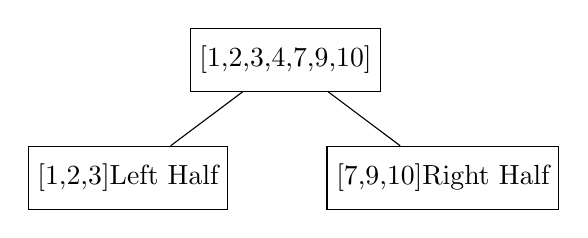
\begin{tikzpicture}[
    level distance=1.5cm,
    sibling distance=4cm,
    every node/.style={draw, rectangle, minimum height=0.8cm, text centered}
]
\node {[1,2,3,4,7,9,10]}
    child {node {[1,2,3]\\Left Half}}
    child {node {[7,9,10]\\Right Half}};
\end{tikzpicture}
\end{center}

Mid = $0 + \frac{6-0}{2} = 3$

\subsection{Step 3: Recursive Calls}

\textbf{Left Half:} $findClosestPairDC([1,2,3,4,7,9,10], 0, 3, 11)$
\begin{itemize}
    \item Further splits into $[1,2]$ and $[3,4]$
    \item Best pair from left: $(3,4)$ with sum $7$, diff $= |7-11| = 4$
\end{itemize}

\textbf{Right Half:} $findClosestPairDC([1,2,3,4,7,9,10], 4, 6, 11)$
\begin{itemize}
    \item Further splits into $[7]$ and $[9,10]$
    \item Best pair from right: $(9,10)$ with sum $19$, diff $= |19-11| = 8$
\end{itemize}

\subsection{Step 4: Cross Pair Analysis}

$findClosestCrossPair([1,2,3,4,7,9,10], 0, 3, 6, 11)$

\textbf{Two-pointer traversal:}
\begin{center}
\begin{tabular}{|c|c|c|c|c|c|}
\hline
\textbf{i} & \textbf{j} & \textbf{arr[i]} & \textbf{arr[j]} & \textbf{sum} & \textbf{diff} \\
\hline
3 & 4 & 4 & 7 & 11 & 0 \\
\hline
\end{tabular}
\end{center}

Since sum = target, this is the optimal cross pair: $(4,7)$

\subsection{Step 5: Final Selection}

$getBestPair(leftPair, rightPair, crossPair, 11)$:
\begin{itemize}
    \item Left pair: $(3,4)$, diff = $4$
    \item Right pair: $(9,10)$, diff = $8$  
    \item Cross pair: $(4,7)$, diff = $0$ ← \textbf{Winner}
\end{itemize}

\textbf{Result:} $(4,7)$ with sum exactly equal to target $11$.

\section{Algorithm Correctness Proof}

\begin{theorem}[Correctness of ClosestPairFinder]
The ClosestPairFinder algorithm correctly finds the pair with sum closest to the target.
\end{theorem}

\begin{proof}
We prove by strong induction on the array size $n$.

\textbf{Base Case:} For $n = 2$, the algorithm returns the only possible pair, which is trivially correct.

\textbf{Inductive Step:} Assume the algorithm works correctly for all arrays of size $< n$. For an array of size $n$:

\begin{enumerate}
    \item The optimal pair falls into exactly one of three categories:
    \begin{itemize}
        \item Both elements in left half
        \item Both elements in right half  
        \item One element in each half
    \end{itemize}
    
    \item By the inductive hypothesis, the recursive calls correctly find the optimal pairs in the left and right halves.
    
    \item The cross pair function uses the two-pointer technique on the sorted array, which examines all relevant cross pairs due to the monotonic property of sums.
    
    \item The getBestPair function correctly selects the minimum among the three candidates.
\end{enumerate}

Therefore, the algorithm returns the globally optimal pair.
\end{proof}

\section{Comparison with Alternative Approaches}

\subsection{Brute Force Approach}

\begin{lstlisting}[caption=Brute Force Solution]
public static int[] bruteForce(int[] arr, int target) {
    int[] bestPair = new int[2];
    int minDiff = Integer.MAX_VALUE;
    
    for (int i = 0; i < arr.length; i++) {
        for (int j = i + 1; j < arr.length; j++) {
            int diff = Math.abs(arr[i] + arr[j] - target);
            if (diff < minDiff) {
                minDiff = diff;
                bestPair[0] = arr[i];
                bestPair[1] = arr[j];
            }
        }
    }
    return bestPair;
}
\end{lstlisting}

\textbf{Complexity:} $O(n^2)$ time, $O(1)$ space

\subsection{Two-Pointer Approach (Without Divide-and-Conquer)}

\begin{lstlisting}[caption=Simple Two-Pointer Solution]
public static int[] twoPointer(int[] arr, int target) {
    Arrays.sort(arr);  // O(n log n)
    int left = 0, right = arr.length - 1;
    int[] bestPair = new int[2];
    int minDiff = Integer.MAX_VALUE;
    
    while (left < right) {
        int sum = arr[left] + arr[right];
        int diff = Math.abs(sum - target);
        
        if (diff < minDiff) {
            minDiff = diff;
            bestPair[0] = arr[left];
            bestPair[1] = arr[right];
        }
        
        if (sum < target) left++;
        else right--;
    }
    return bestPair;
}
\end{lstlisting}

\textbf{Complexity:} $O(n \log n)$ time, $O(1)$ space

\subsection{Performance Comparison}

\begin{center}
\renewcommand{\arraystretch}{1.5}
\begin{tabular}{|l|c|c|c|}
\hline
\textbf{Approach} & \textbf{Time Complexity} & \textbf{Space Complexity} & \textbf{Pros/Cons} \\
\hline
Brute Force & $O(n^2)$ & $O(1)$ & Simple but slow \\
Two-Pointer & $O(n \log n)$ & $O(1)$ & Optimal and simple \\
Divide-Conquer & $O(n \log n)$ & $O(\log n)$ & Educational value \\
\hline
\end{tabular}
\end{center}

\section{Edge Cases and Error Handling}

\subsection{Input Validation}

The algorithm handles several edge cases:

\begin{enumerate}
    \item \textbf{Null array:} Returns null immediately
    \item \textbf{Array with < 2 elements:} Returns null (no pair possible)
    \item \textbf{Empty array:} Covered by length check
    \item \textbf{Single element:} Covered by length check
\end{enumerate}

\subsection{Numerical Considerations}

\begin{itemize}
    \item \textbf{Integer overflow:} The algorithm uses int arithmetic; for very large numbers, consider using long
    \item \textbf{Integer.MAX_VALUE:} Used as initial comparison value; ensure target differences don't exceed this
\end{itemize}

\section{Optimizations and Variations}

\subsection{Possible Optimizations}

\begin{enumerate}
    \item \textbf{Early termination:} If exact target sum is found, return immediately
    \item \textbf{Iterative implementation:} Reduce space complexity by eliminating recursion
    \item \textbf{Parallel processing:} Left and right recursive calls can be parallelized
\end{enumerate}

\subsection{Variations}

\begin{enumerate}
    \item \textbf{k-closest pairs:} Modify to return top k pairs
    \item \textbf{Weighted pairs:} Include weights in the optimization function
    \item \textbf{Multiple targets:} Find pairs closest to any of several targets
\end{enumerate}

\section{Conclusion}

The ClosestPairFinder algorithm demonstrates an elegant application of the divide-and-conquer paradigm to solve the closest pair sum problem. While a simpler two-pointer approach exists with the same time complexity, this implementation showcases important algorithmic concepts:

\begin{itemize}
    \item \textbf{Problem decomposition:} Breaking complex problems into manageable subproblems
    \item \textbf{Recursive thinking:} Solving problems by reducing to smaller instances
    \item \textbf{Efficient combination:} Merging subproblem solutions optimally
\end{itemize}

The algorithm achieves optimal $O(n \log n)$ time complexity and demonstrates the power of combining sorting with divide-and-conquer techniques. This approach is particularly valuable for educational purposes and serves as a foundation for more complex geometric and optimization algorithms.

\subsection{Key Takeaways}

\begin{enumerate}
    \item Sorting enables efficient searching and optimization
    \item Divide-and-conquer provides systematic problem-solving approach
    \item Two-pointer technique leverages sorted array properties
    \item Careful base case handling ensures algorithm correctness
\end{enumerate}

\vfill
\begin{center}
\rule{\textwidth}{1pt}
\vspace{0.5em}
\textit{Algorithm Analysis and Implementation Guide}\\
\textbf{ClosestPairFinder Documentation} | \today
\vspace{0.5em}
\rule{\textwidth}{1pt}
\end{center}

\end{document}
